\documentclass[10pt]{article}
%\usepackage[french]{babel}
\usepackage{fontspec}
\usepackage{polyglossia}
\setdefaultlanguage{french}
\usepackage[a4paper,margin=2cm]{geometry}
\usepackage{url,hyperref}
%\usepackage{siunitx}
%\usepackage{schemabloc}
%\usepackage{listings}
%\usepackage{auto-pst-pdf}
%\usepackage{pst-circ}
%\usepackage{soul}
%\usepackage{verbatim}
\usepackage{lmodern}
%\usepackage{tikz}
%\usepackage[european,cuteinductors,siunitx]{circuitikz}
\usepackage{xunicode,xltxtra}
\usepackage{graphicx}
%\usepackage{amsmath}
\usepackage{minted}
%\usepackage{multicol}
\title{
\includegraphics{inp-enseeiht} \\ ~ \\ ~ \\ ~ \\ ~ \\ Exercices de Matlab \\ ~ \\ Troisième séance \\ ~  \\ Structures de Contrôle \\ Équations différentielles Ordisnaires}
\author{Guilhem Saurel}
\date{\today}
\renewcommand{\thesubsection}{\thesection .\Alph{subsection}}
\begin{document}

 \begin{titlepage}
  \maketitle
  \tableofcontents
 \end{titlepage}

 \section{Abaque de Smith}
  \inputminted[linenos]{matlab}{abaque_de_smith.m}
  \begin{center}
   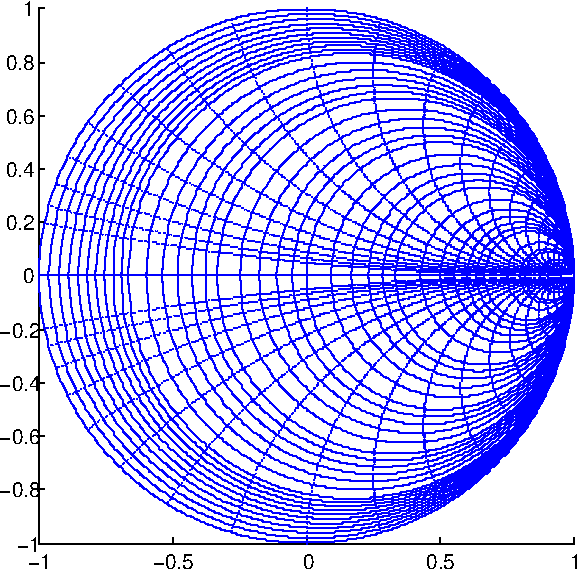
\includegraphics{abaque_de_smith}
  \end{center}
  \newpage

 \section{Équations Différentielles Ordinaires}
  \subsection{Modules Euler, RK2 \& RK4}
   \inputminted[linenos]{matlab}{eul.m}
   \inputminted[linenos]{matlab}{RK2.m}
   \inputminted[linenos]{matlab}{RK4.m}

  \subsection{Résolution par les trois méthodes}
   \inputminted[linenos]{matlab}{resolution.m}
   \begin{center}
    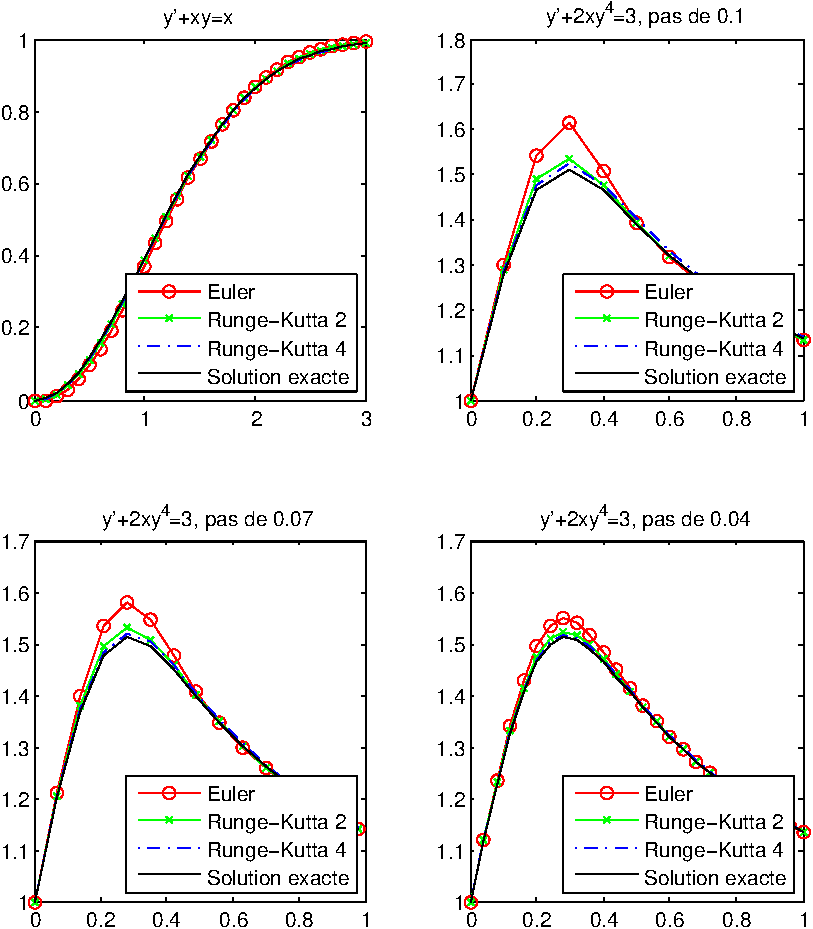
\includegraphics{EquaDiffs}
   \end{center}


\end{document}
